\documentclass{article}[12 pt]
\usepackage[utf8]{inputenc}
\setlength\parindent{0pt}
\usepackage[margin=2.5cm]{geometry}
\usepackage{hyperref}
\usepackage{setspace}
\pagenumbering{arabic}
\usepackage{graphicx}
\usepackage[super]{nth}
\usepackage{amsmath} 
\usepackage{subfigure}

\hypersetup{
  colorlinks   = true, 
  urlcolor     = blue,
  linkcolor    = black,
  citecolor   = black}
\usepackage{fancyhdr}




\begin{document}
\title{Parameters}
\author{Emma Holmes}
\date{\today}

\maketitle

\section{Initial conditions of the model}
\onehalfspacing
\begin{center}
\begin{tabular}{ l l l} 
\hline
Symbol & Initial condition & Variable description \\
\hline
$\lambda(0)$ & 0.675 & Employment rate \\
$\omega(0)$ & 0.578 & Wage share  \\
$d(0)$ & 1.53 & Debt share \\
\hline 
$K(0)$ & 161.3 & Capital stock \\
$w(0)$ & 10.591 & Wages \\
$D(0)$ & 91.4 & Debt in trillions of USD\\
$a(0)$ & 18.323 & Labour productivity \\ 
$N(0)$ & 4.83 & Workforce in billions \\
$\sigma(0)$ & 0.62 &  Emission intensity of the economy \\
$g_{\sigma}(0)$ & -0.0105 & Growth rate of the emissions intensity of the economy  \\
$p(0)$ & 1 & Composite good price level \\
$p_{BS}(0)$ & 547.22 & Price level of backstop technology  \\
$p_{c}(0)$ & 2 & Carbon price  \\
$E_{land}(0)$ & 2.6 & Exogenous land use CO$_2$-e emissions, in Gt C  \\
$CO_2^{AT}(0)$ & 851 & CO$_2$-e concentration in the atmosphere layer, in Gt C \\
$CO_2^{UP}(0)$ & 460 & CO$_2$-e concentration in the biosphere and upper ocean layer, in Gt C \\
$CO_2^{LO}(0)$ & 1740 & CO$_2$-e concentration in the lower ocean layer, in Gt C  \\
$T(0)$ & 0.85 & Temperature anomaly, in degrees Celsius  \\
$T_{LO}(0)$ & 0.0068 & Temperature anomaly in lower ocean layer, in degrees Celsius \\
\hline
\end{tabular}
\end{center}

%* $n = (p_c / p_{BS})^{1/(\theta-1)}$ implies $p_c = p_{BS} * n^{\theta -1}$ or if we are using a subsidy as in Debt and Damages: $n = (p_c /(1-s) p_{BS})^{1/(\theta-1)}$ implies $p_c = p_{BS} * (1-s) * n^{\theta -1}$ .


Initial conditions explored: $0 \leq \lambda(0) \leq 1, \, 0 \leq \omega(0) \leq 1, \, \text{and} \, 0 \leq d(0) \leq 3$ while $\bar \gamma =0.9$, $\bar \eta = 0.192$, and $\bar \xi = \{ 1.18, 1.3, 1.875\}$.



\section{Model parameters}
\begin{tabular}{ l l l } 
\hline
Symbol & Value & Parameter description \\
\hline
$\bar \alpha$ & 0.02 & Productivity growth rate  \\ 
$\bar \delta$ & 0.04 & Depreciation rate of capital \\
$\bar \nu$ & 2.7  & Capital to output ratio \\
$\bar \delta_N $ & 0.031 & Growth rate of workforce\\
$ \bar N_{max} $ & 7.056 & Maximum workforce \\
$\Phi_0$ & -0.292 & Phillips curve constant -- linear specification \\
$\Phi_1$ & 0.469 & Phillips curve slope -- linear specification \\
$\kappa_0$ & 0.032 & Investment function constant \\
$\kappa_1$ & 0.575 & Investment  function slope \\
$\kappa_{min}$ & 0  & Investment  function minimum \\
$\kappa_{max}$ & 0.3 & Investment  function maximum \\
$\Delta_0$ & -0.078 & Dividend function constant \\
$\Delta_1$ & 0.553 & Dividend function slope \\
$\Delta_{min}$ & 0  & Dividend function minimum \\
$\Delta_{max}$ & 0.3 & Dividend function maximum \\
$r$ & 0.02 & Long term interest rate \\
$\bar \eta$  & 0.192 & Inflation relaxation parameter\\
$\bar \xi$ & 1.875 & Price markup \\
$\bar \gamma$ & 0.9 & Effect of inflation on wages \\
$C^{AT}_{preind}$ & 588 & Preind. concentration of CO$_2$ in the atmosphere layer, in Gt C \\
$C^{UP}_{preind}$  & 360 & Preind. concentration of CO$_2$ in the biosphere/upper ocean layer, in Gt C \\
$C^{LO}_{preind}$ & 1720 & Preind. concentration of CO$_2$ in the lower ocean layer, in Gt C   \\
$\phi_{12}$  & 0.024 & Transfer coefficient for carbon from AT to UP\\
$\phi_{23}$ & 0.001 & Transfer coefficient for carbon from UP to LO\\
$\delta_{g_{\sigma}}$  & -0.001 & Variation rate of the growth of emission intensity \\
$\delta_{E_{land}}$ & -0.022 & Growth rate of land use change CO2-e emissions  \\
$F_{dbl}$ & 3.682 & Change in radiative forcing from a doubling of preindustrial CO$_2$, in W/m$^2$  \\
$F_{exo}^{start}$ & 0.5 & Initial value of exogenous radiative forcing \\
$F_{exo}^{end}$ & 1 & End value of exogenous radiative forcing \\
$T_{preind}$ & 13.74 & Preindustrial temperature, in degrees Celsius \\
$C_{init}$ & 10.20 & Heat capacity of AT and UP, in SI \\
$C_{LO}$ & 3.52 & Heat capacity of the lower ocean layer \\
$\gamma^*$ & 0.0176 & Heat exchange coefficient between temperature layers, in SI \\
$S$ & 3.1 & Equilibrium climate sensitivity, in degrees Celsius \\
$\xi_1$ & 0 & Damage function parameter \\
$\xi_2$ & 0.00236 & Damage function parameter  \\
$\xi_3$ & 4.48e-06 & Damage function parameter \\
$\zeta$ & 7 & Damage function parameter \\
$\theta$ & 2.6 & Abatement cost function parameter \\
$g_{p_{BS}}$ & -0.0051 & Growth rate of the price of backstop technology \\
$\delta_C$ & 1 & Linear growth rate of the carbon price \\
\hline
\end{tabular}


\newpage 

Parameter space explored: $0 \leq \bar \eta \leq 1, \, 1 \leq \bar \xi \leq 2.5, \, \text{and} \, 0 \leq \bar \gamma \leq 1$.

\subsection{Parameter distributions}
Here I compare the distributions (red lines) to the data you sent me (histograms).

% \begin{figure}[h]
%     \centering
%     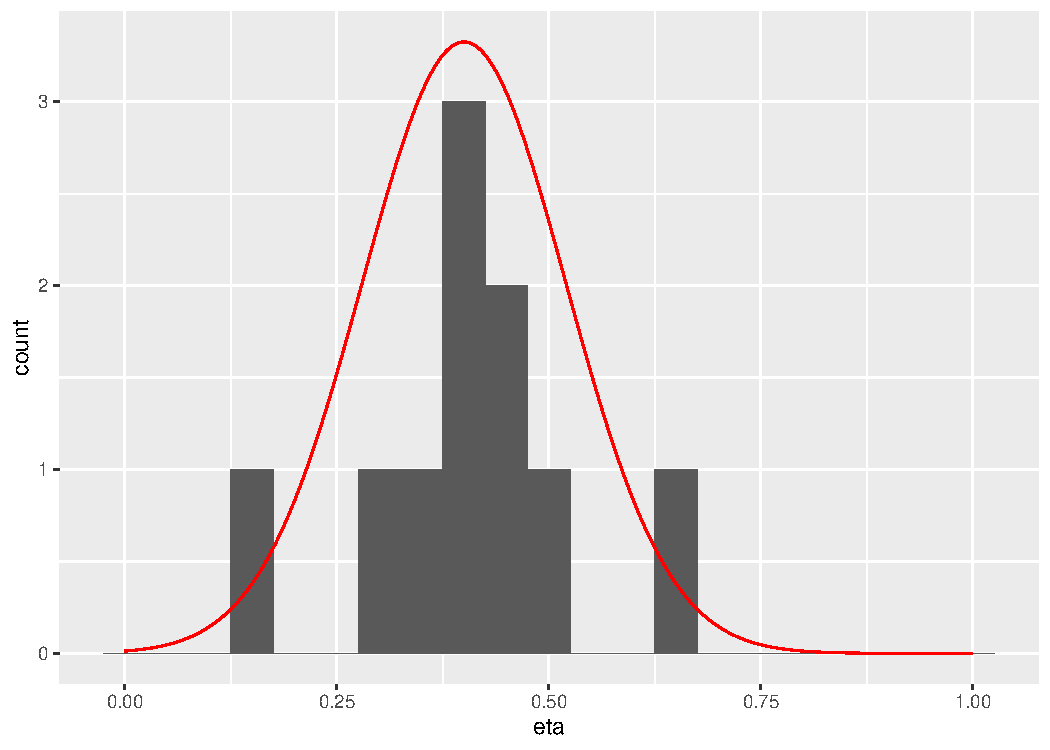
\includegraphics[ width=11.5cm]{eta_dist.pdf}
%     \caption{Distribution of $\bar \eta$ (in red) compared to a histogram of the estimated values.}
%     \label{fig:my_label}
% \end{figure}

% \begin{figure}
%     \centering
%     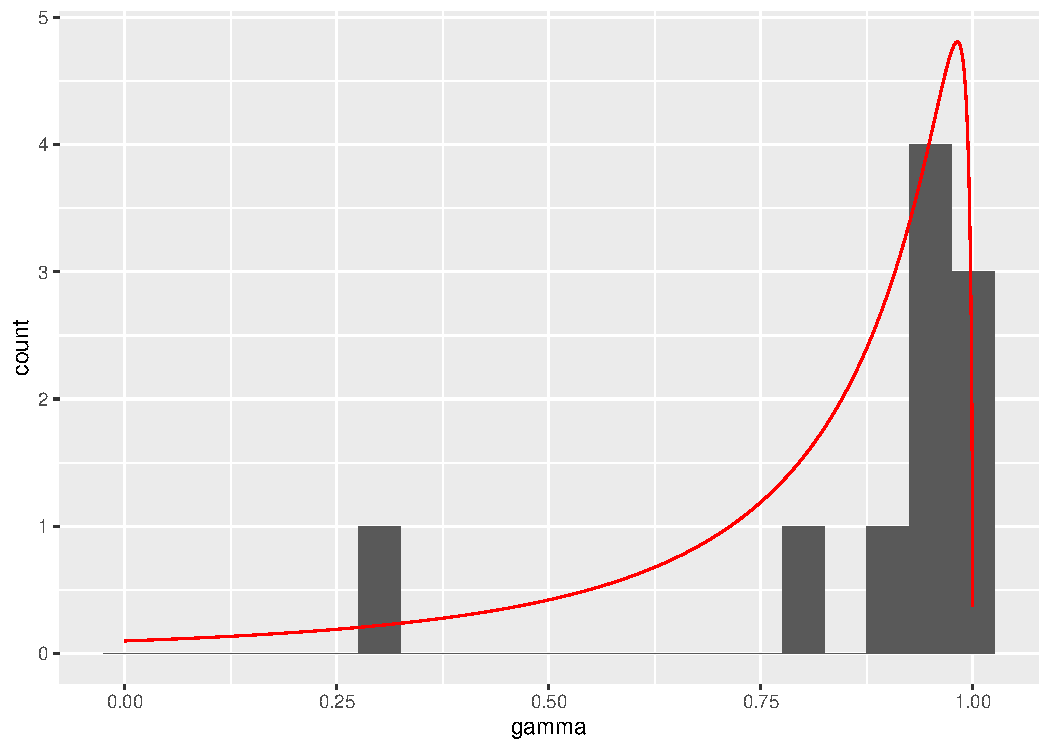
\includegraphics[ width=11.5cm]{gamma_dist.pdf}
%     \caption{Distribution of $\bar \gamma$ (in red) compared to a histogram of the estimated values.}
%     \label{fig:my_label}
% \end{figure}


% \begin{figure}
%     \centering
%     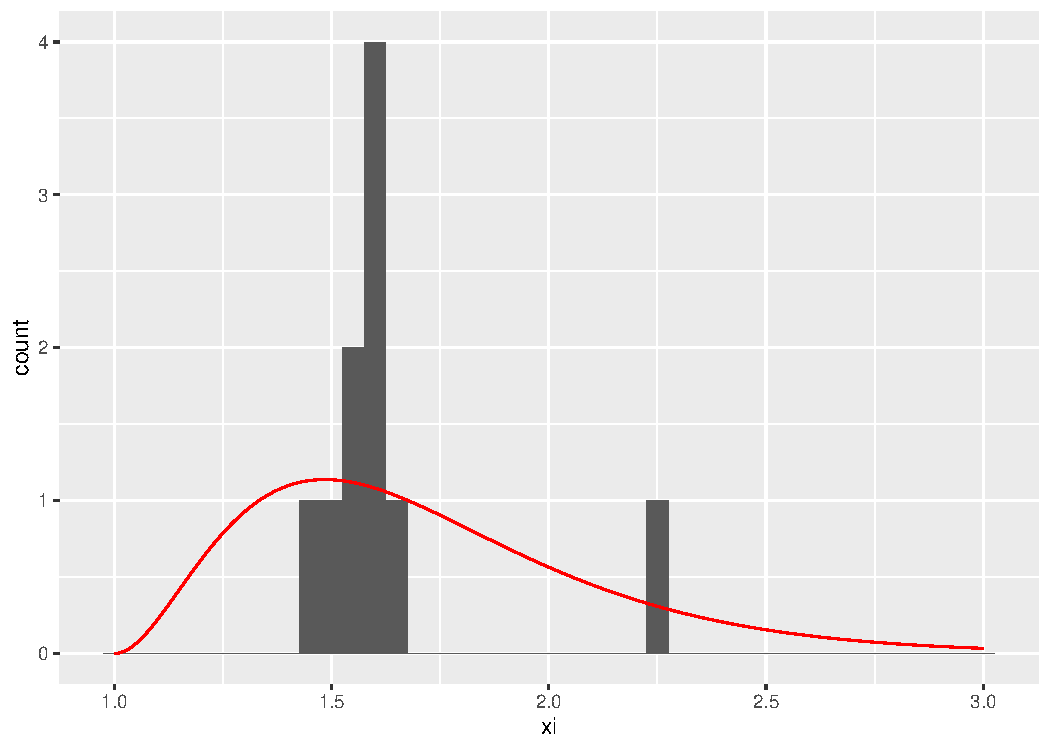
\includegraphics[ width=11.5cm]{xi_dist.pdf}
%     \caption{Distribution of $\bar \xi$ (in red) compared to a histogram of the estimated values. The generalized gamma distribution was chosen because values $\xi < 1$ are not permitted.}
%     \label{fig:my_label}
% \end{figure}


\begin{figure}[hpt]
\centering    
\subfigure[Distribution of the relaxation parameter, $\eta$]{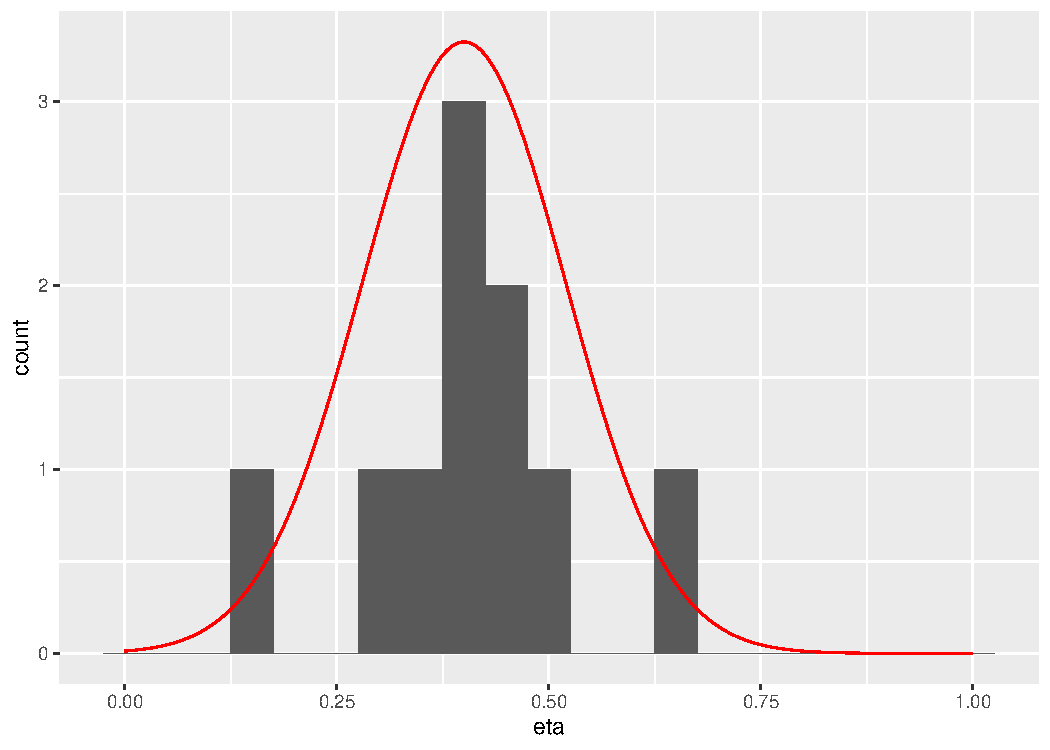
\includegraphics[width=8cm]{eta_dist.pdf}}
\subfigure[Distribution of the money illusion parameter, $\gamma$]{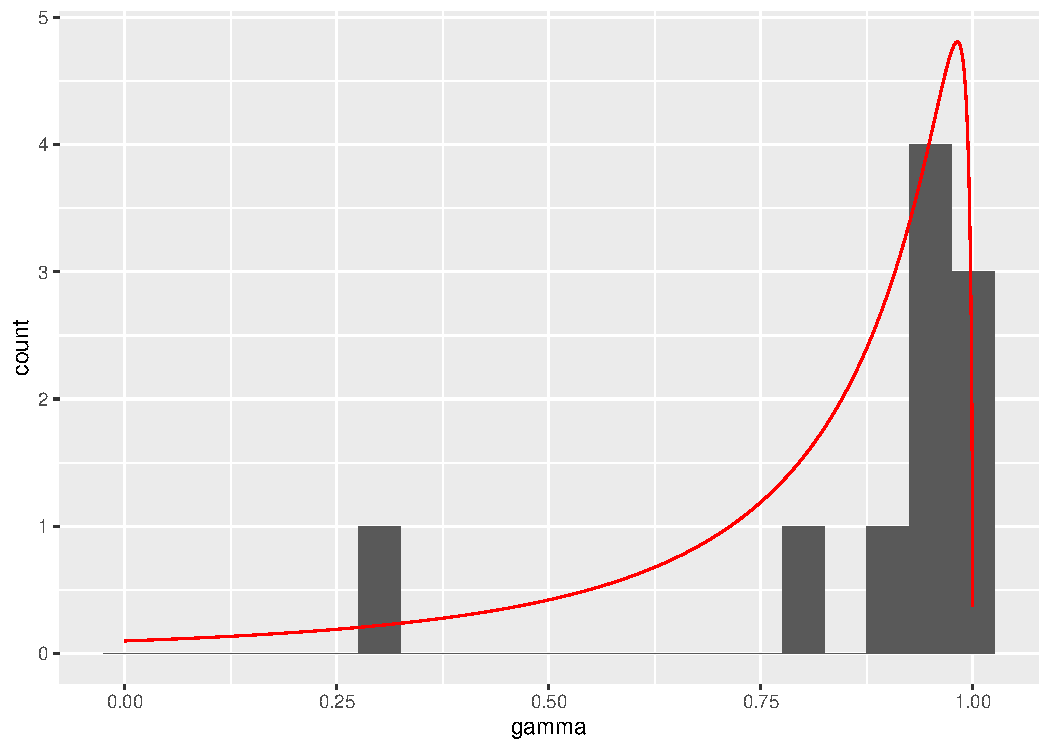
\includegraphics[width=8cm]{gamma_dist.pdf}}
\subfigure[Distribution of the markup rate, $\xi$]{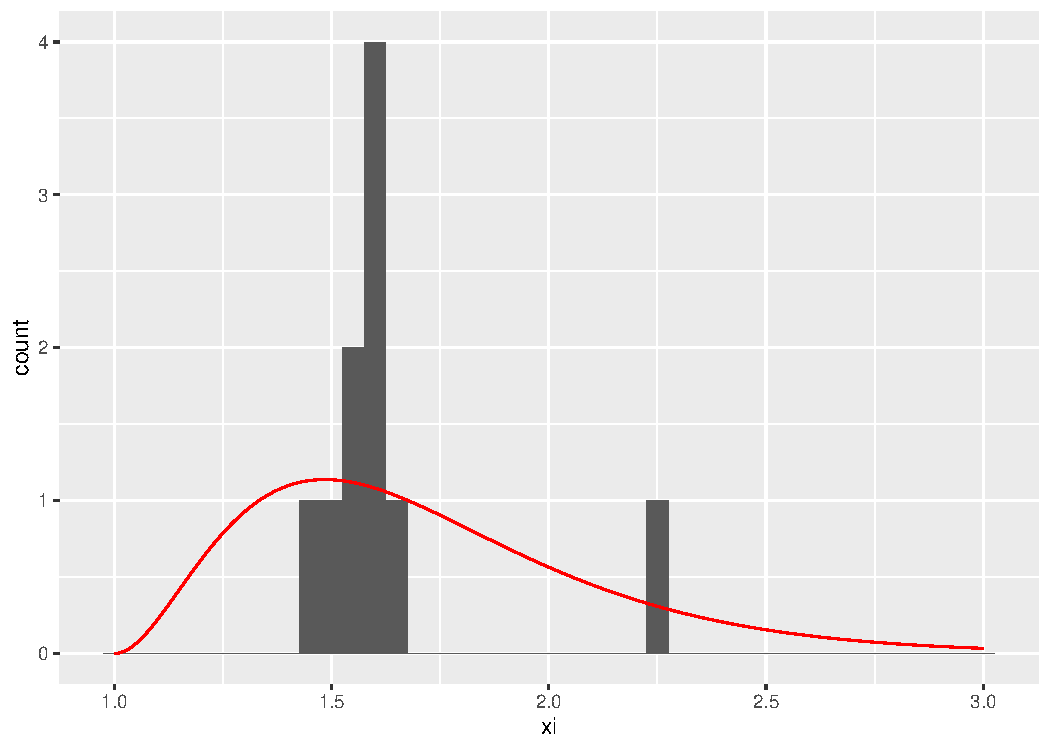
\includegraphics[width=8cm]{xi_dist.pdf}}
\caption{Probability density functions of the pricing parameters $\eta$, $\xi$, and $\gamma$.}
\label{fig:distributionsl}
\end{figure}

\end{document}
